\section{Teori Informasi: Entropi dan Laju Bahasa}

\subsection{Entropi}

\textbf{Entropi} dalam teori informasi Shannon mengukur ketidakpastian atau kandungan informasi dari suatu sumber data \cite{shannon1949,entropy_wikipedia}. Untuk sumber diskrit dengan probabilitas $p_i$ untuk simbol ke-$i$:
\[
H(X) = -\sum_{i} p_i \log_2 p_i \quad \text{(bit per simbol)}
\]
Entropi maksimum tercapai ketika semua simbol berpeluang sama. Untuk alfabet 26 huruf Inggris, entropi maksimum teoritis ialah $\log_2 26 \approx 4{,}7$ bit per huruf.

Claude Shannon dalam makalah ``Communication Theory of Secrecy Systems'' (1949) menerapkan prinsip teori informasi pada sistem kriptografi, menandai peralihan kriptografi klasik ke kriptografi modern berbasis sains \cite{shannon1949}. Konsep \textit{equivocation} (berbasis entropi) dipakai untuk menganalisis keamanan teoretis cipher. Shannon juga memperkenalkan prinsip confusion dan diffusion yang hingga kini menjadi landasan desain cipher modern.

\begin{table}[htbp]
\centering
\small
\begin{tabular}{|l|c|c|}
\toprule
\textbf{Alfabet} & \textbf{Jumlah Simbol} & $H_{\max}$ (bit/simbol) \\
\midrule
Biner & 2 & 1 \\
Desimal & 10 & $\approx 3{,}32$ \\
Inggris (A--Z) & 26 & $\approx 4{,}70$ \\
ASCII (printable) & 95 & $\approx 6{,}57$ \\
\bottomrule
\end{tabular}
\caption{Entropi maksimum untuk beberapa alfabet.}
\end{table}

\subsection{Laju Bahasa dan Redundansi}

\textbf{Laju bahasa} (rate of language) ialah rata-rata bit informasi per karakter dalam teks nyata suatu bahasa. Karena distribusi huruf tidak seragam (misalnya E dan A lebih sering daripada Q dan Z), laju bahasa Inggris nyata sekitar 1{,}0--1{,}5 bit per karakter, lebih rendah dari entropi maksimum.

\textbf{Redundansi} didefinisikan sebagai $R = 1 - H/L$, dengan $H$ entropi aktual dan $L$ entropi maksimum. Redundansi bahasa Inggris diperkirakan sekitar 75\%; artinya teks masih dapat dipahami meskipun banyak huruf hilang atau salah. Redundansi inilah yang memungkinkan \textit{analisis frekuensi} berhasil memecah cipher substitusi monoalfabetik.

Pemahaman entropi dan redundansi penting dalam kriptanalisis: cipher yang ideal seharusnya menghasilkan ciphertext dengan entropi tinggi dan redundansi rendah sehingga penyerang sulit memanfaatkan pola bahasa. One-Time Pad mencapai keamanan sempurna karena ciphertextnya tidak mengandung redundansi plaintext asli.

\begin{figure}[htbp]
\centering
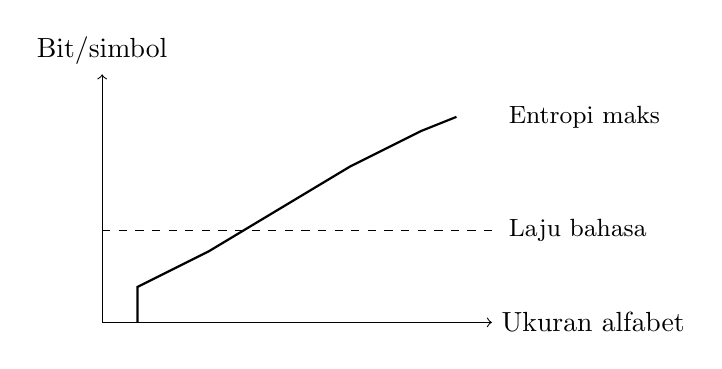
\begin{tikzpicture}[scale=0.9]
  \draw[->] (0,0) -- (5.5,0) node[right] {Ukuran alfabet};
  \draw[->] (0,0) -- (0,3.5) node[above] {Bit/simbol};
  \draw[thick] (0.5,0) -- (0.5,0.5) -- (1.5,1) -- (2.5,1.6) -- (3.5,2.2) -- (4.5,2.7) -- (5,2.9);
  \draw[dashed] (0,1.3) -- (5.5,1.3);
  \node[right, font=\small] at (5.6,2.9) {Entropi maks};
  \node[right, font=\small] at (5.6,1.3) {Laju bahasa};
\end{tikzpicture}
\caption{Ilustrasi: entropi maksimum naik dengan ukuran alfabet; laju bahasa aktual lebih rendah karena redundansi.}
\end{figure}
